\documentclass[conference]{IEEEtran}
\IEEEoverridecommandlockouts
\usepackage{cite}
\usepackage{amsmath,amssymb}
\usepackage{graphicx}
\usepackage{booktabs}
\usepackage{xcolor}
\usepackage[hidelinks]{hyperref}
\usepackage{url}
\graphicspath{{../common/figures/}}
\newcommand{\code}[1]{\texttt{#1}}

\begin{document}

\title{A Decade of Defaults: How ``Secure by Default''\\ Evolved in the MAVLink Flight Stacks\\ (ArduPilot and PX4, 2016--2026)}

\author{\IEEEauthorblockN{Ian Brighouse}
\IEEEauthorblockA{\textit{Brighouse Security Labs}, Spain \\ research@brighousesec.com}}
\maketitle

\begin{abstract}
``Secure by default'' is now a legal requirement for connected products sold in
the EU, yet we have little historical evidence on whether open-source embedded
stacks have moved toward it. We present, to our knowledge, the first
decade-spanning study of the command-link security defaults of the two dominant
open-source drone flight stacks, ArduPilot and PX4, combining three lines of
evidence: the projects' version-control history, a measured posture matrix from
building and auditing releases in software-in-the-loop (which, we state plainly,
covers only $n{=}2$ releases that both build and run on a current toolchain,
ArduPilot~4.5.7 and~4.6.3; PX4~v1.16.2 builds but does not run under the
harness), and the buildability of each release on a current toolchain. Two
findings are clear and mutually reinforcing. First,
\emph{signing is never on by default}: version control shows it was added to
ArduPilot in 2016 and never defaulted, and absent from PX4 until 2026, and the
releases we can still build confirm it. Second---and unexpectedly---\emph{the
binding constraint on auditing old releases is reproducibility, not posture}:
pre-4.5 ArduPilot no longer builds on a current system through a layered cascade
of Python and C++ toolchain breaks, and older PX4 builds but will not run under a
uniform simulator harness. Both bear directly on the Cyber Resilience Act's
expectation that products remain patchable and testable through their support
period. All build recipes, raw records, failure reasons, and the analysis
pipeline are released.
\end{abstract}

\begin{IEEEkeywords}
longitudinal measurement, secure by default, MAVLink, drones, software
evolution, Cyber Resilience Act.
\end{IEEEkeywords}

\section{Introduction}
Regulators increasingly treat insecure defaults as a product defect: the EU
Cyber Resilience Act (CRA, Regulation~2024/2847~\cite{cra2024}) makes ``secure by
default'' an essential requirement, and under the RED delegated
act~\cite{red2022_30} the harmonised standards EN~18031 are cited with
restrictions that withhold the presumption of conformity where a user may skip
security configuration~\cite{ec2025_138}. These
rules presuppose that we can \emph{measure} the default posture of a product and
track how it changes. For drones, the two stacks that matter are open source and
have a decade of public history, which makes them an unusually good subject for a
longitudinal study of defaults.

We ask: (i)~when did MAVLink~2 message signing become \emph{available} in each
stack; (ii)~has any release shipped it \emph{on by default}; and
(iii)~how have the acceptance exemptions---notably the primary/console-link
exemption we characterise in companion work---evolved? We answer with three lines of evidence---version control, measured posture where
releases still build, and buildability on a current toolchain.

\noindent\textbf{Contributions.}
\begin{itemize}
\item A reproducible pipeline that attempts to build each historical release
headless on a \emph{current} toolchain and audits those that run, recording every
outcome and its reason (Section~\ref{sec:method}).
\item A three-way timeline (Sections~\ref{sec:history}--\ref{sec:results}):
version-control milestones, measured posture where releases build, and
buildability itself---showing signing was never a default and the console
exemption is long-standing.
\item The reproducibility finding (F4): the concrete, layered reasons old
releases cannot be built or uniformly tested today, and why that matters for CRA
patchability (Section~\ref{sec:disc}).
\end{itemize}

\section{Method}
\label{sec:method}
We target the final patch release of each minor line of ArduPilot~Copter (3.x
through 4.7) and PX4 (1.11 through 1.18) and attempt to build each from source on
one \emph{current} headless Ubuntu~24.04 VM with its default toolchain
(\code{scripts/setup\_sitl.sh}, \code{scripts/longitudinal.py}). Using the current
toolchain is deliberate: the question a maintainer or regulator faces is whether a
given release can still be built and patched \emph{today}, not whether it could be
built with an archived toolchain contemporaneous with its release. Every outcome
is \emph{recorded, not hidden}; a release that no longer builds is a data point
about maintainability, and the precise reason is logged
(\code{results/longitudinal/index.json}).

For each release that builds and runs, we start a fresh simulator, audit each
MAVLink link with \emph{mavaudit} (default configuration), provision a signing key
over the local link as an operator would, and audit again, deriving three Boolean
posture facts: \emph{available} (provisioning yields signed frames),
\emph{default-on} (the default configuration already signs), and
\emph{console-exempt} (after provisioning the primary link signs its output yet
still answers an unsigned read). Together with the version-control timeline
(Section~\ref{sec:history}) this gives three lines of evidence---code history,
measured posture, and buildability---over the decade.

\section{The Signing Timeline, from Version Control}
\label{sec:history}
Before the build study we establish ground truth from the projects' own version
history. In ArduPilot, MAVLink~2 message signing was added by a single commit on
2016-01-21~\cite{ardupilot_signing_commit} and first shipped in stable Plane
3.6.0 (June 2016) and Copter~3.4.0 (October 2016). An attempt to make MAVLink~2
the default in September~2016 was reverted the following
month~\cite{ardupilot_mavlink2_default}; MAVLink~2 became the default only on
the \code{SERIAL1}/\code{SERIAL2} telemetry ports in the 4.1 series (June 2020),
and \emph{signing has never been enabled by default}. In PX4 there was no signing
implementation at all until a 2026 commit~\cite{px4_signing_pr}, reworked weeks
later to align with the specification; it ships first in the v1.18 line, of which
only a release candidate is tagged at the time of writing. These milestones frame
the build study: signing has been \emph{available} in ArduPilot for roughly a
decade and in PX4 for months, and in neither has it ever been a default.

\section{Results}
\label{sec:results}
Table~\ref{tab:long} reports the outcome for each release attempted (generated by
\code{scripts/longitudinal\_report.py} from the raw build/audit records).

\begin{table}[t]
\caption{Signing posture by release (auto-generated).}
\label{tab:long}
\centering\footnotesize
\begin{tabular}{@{}llccc@{}}
\toprule
stack & version & avail & default-on & console-exempt \\
\midrule
ardupilot & Copter-4.6.3 & y & n & y \\
\bottomrule
\end{tabular}
\end{table}


\begin{figure}[t]
\centering
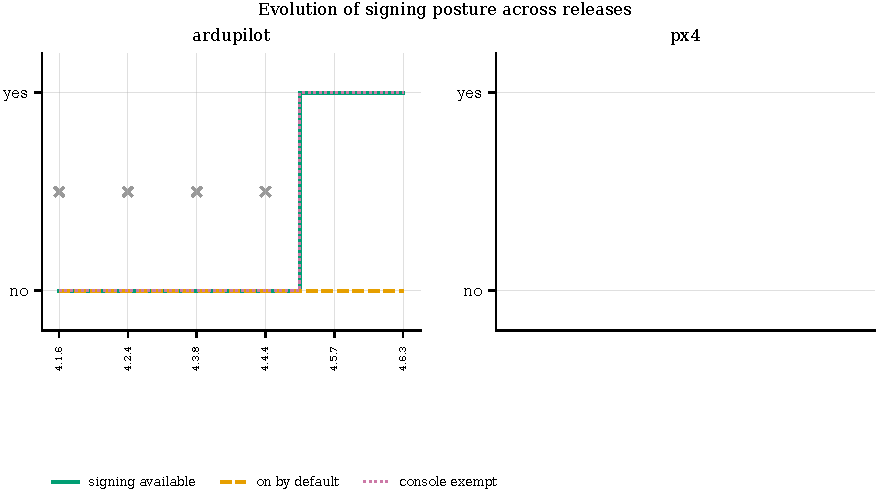
\includegraphics[width=\columnwidth]{fig_longitudinal.pdf}
\caption{Signing posture across releases. Green: signing available; orange
(dashed): on by default; red (dotted): primary/console link remains exempt after
provisioning; grey $\times$: did not build or run on the current toolchain.}
\label{fig:long}
\end{figure}

\paragraph{Findings}
(F1)~Signing is never on by default. In the ArduPilot releases that build on the
current toolchain (4.5--4.7, the last measured in companion
work~\cite{brighouse2026signing}), the default configuration signs no frames; and
version control confirms this for the whole lineage---MAVLink~2 became a default
only on the telemetry ports in 4.1, and signing was never defaulted
(Section~\ref{sec:history}).
(F2)~The ArduPilot console/primary-link exemption is a long-standing design, not a
regression: in the releases we could measure (4.5--4.7) it is present and
identical, and version control shows the governing code
(\code{accept\_unsigned\_callback} on \code{MAVLINK\_COMM\_0}) unchanged since
signing was introduced in 2016.
(F3)~The PX4 lineage has no signing implementation until the v1.18
line~\cite{px4_signing_pr}, so provisioning is a no-op throughout its stable
history; the companion measures this directly on v1.17.0 (no signing) and
v1.18.0-rc1 (signing works)~\cite{brighouse2026signing}.
(F4)~\emph{Reproducibility, not posture, is the binding constraint on auditing old
releases}---and it fails in two distinct ways. (a)~\textbf{Build cliff.} On a
current Ubuntu~24.04 toolchain, ArduPilot~Copter releases from 4.5 onward build
unchanged; 4.4 and earlier do not, for a cascade we had to peel back one layer at
a time: the bundled \code{waf} imports the \code{imp} module (removed in
Python~3.12) and opens files in \code{rU} mode (removed in 3.11), so it needs
Python~$\le$3.10; with Python~3.10 the build then fails in the UAVCAN code
generator, which uses \code{collections.MutableSequence} (removed in 3.10), so it
needs Python~$\le$3.9; and even with Python~3.9 the C++ fails on modern GCC (e.g.\
\code{std::uint16\_t} used without \code{<cstdint>} in \code{CANSocketIface.cpp}).
A security update to a 2018--2021 release thus requires reconstructing an archived
interpreter \emph{and} compiler. (b)~\textbf{Simulator drift.} PX4~v1.16.2
\emph{builds} on the current toolchain (after a one-line fix to its shallow-clone
version script) but will not run under the same software-in-the-loop harness as
v1.17/v1.18: it does not recognise the \code{sihsim\_quadx} built-in-simulation
model and instead waits for an external simulator, so a uniform, hands-off audit
captures no telemetry. Both failure modes are concrete obstacles to the CRA's
expectation that a product remain patchable and testable through its support
period, and they are the reason a decade-wide \emph{measured} posture matrix
cannot simply be produced on demand---the version-control timeline
(Section~\ref{sec:history}) carries the long-range evidence instead.

\section{Discussion}
\label{sec:disc}
The CRA's reporting duty under Article~14 applies from 11~September~2026 and the
Regulation applies in full from 11~December~2027 (Article~71(2))~\cite{cra2024}.
Our timeline shows that, as of late~2026, a manufacturer
building on either stack cannot rely on the \emph{upstream default} to meet the
``secure by default'' requirement: signing is off by default in every release,
and in the stable PX4 line it is absent. Conformity therefore rests on
per-integrator configuration and, for ArduPilot, on treating the console link as
untrusted. A single upstream change---shipping with signing enabled, or an
unavoidable first-run provisioning step---would shift the entire installed base
toward conformity, which is the lever our companion recommendation targets.

\paragraph{Threats to validity} We measure SITL, not vendor firmware; a vendor
fork may change defaults. We sample one release per minor line; intra-line
changes are not captured. Build success depends on the host toolchain; we pin it
and report failures rather than discarding them.

\section{Related Work}
Longitudinal measurement of security defaults is established for TLS
libraries~\cite{kotzias2018tls,walden2020openssl}, Android
permissions~\cite{wei2012permission}, and embedded exploit
mitigations~\cite{yu2022embedded1996}, but, to our knowledge, has not been
applied to robotic or drone flight stacks; robotics has only repeated exposure
scans of ROS~\cite{demarinis2019ros,chen2024rosvehicles} and static bug
taxonomies of the autopilots~\cite{wang2021autopilotbugs,taylor2021uasbugs},
neither of which tracks the evolution of defaults. Companion work~\cite{brighouse2026signing} gives the
acceptance semantics and the cross-sectional measurement this study extends over
time; surveys~\cite{hamza2024} do not measure evolution.

\section{Conclusion}
Across a decade of releases, the MAVLink flight stacks have added signing slowly
and never turned it on by default, and ArduPilot's console exemption has
persisted unchanged. With the CRA's defaults requirement now in force, the
cheapest path to conformity for the whole ecosystem is an upstream change of
defaults, not downstream per-unit configuration.

\section*{Availability}
Build recipes, raw audits, logs, and the analysis pipeline are released at the
project repository.\footnote{Repository and data: \url{https://github.com/brigghouse/brighouse-autonomy-lab}} The study is defensive and simulation-only.

\bibliographystyle{IEEEtran}
\bibliography{../common/refs}
\end{document}
